\section{Configuration of the AskoziaPBX}
\label{sec:configuration}

This paragraph is about the configuration of the AskoziaPBX. First of all, the used configfile from Askozia is downloaded because the
user should not have to reconfigure the whole box including all accounts and the dialplan after every test. The target is to deliver
the Askozia box just like it was issued. So, there are three necessary steps which are described in the next chapters.

\begin{figure} [htbp]
\centering
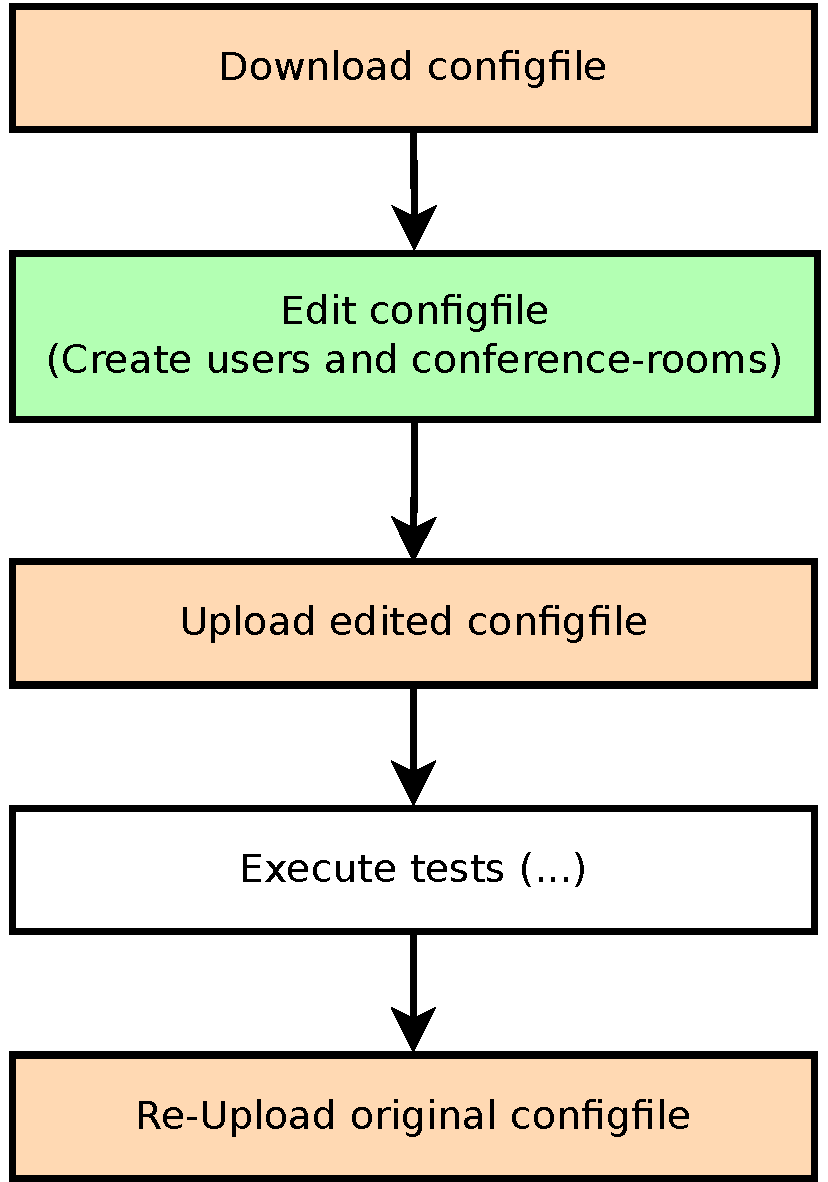
\includegraphics [width=7cm] {config-1}
\caption{Process of editing the Askozia-configfile}
\end{figure}

\subsection{Down-/Upload Configfile}

For downloading the configfile, it is necessary to send a HTML POST request to Askozia. Or, to be more precise, it has to be sent to the qstat-page of the Askozia box. The useragent has to be authenticated as root and the content type must be ``multipart/form-data''. With this POST request, Askozia sends the output of the qstat page. For downloading the configfile, the parameter ``Download'' has to be set to any desired value -- but it has to be set.

In the performance test script, the following perl code is used to send this POST request:
\begin{lstlisting}[breaklines=true,label=code:config-post-request,caption={POST request for downloading configfile} ]
use HTTP::Request::Common;
use LWP;
my $ua = new LWP::UserAgent;
$ua->credentials ("$ask_ip:$ask_port",
	$ask_realm, "$ask_user" => "$ask_pw");
my $res = $ua->request (POST
	"http://$ask_ip:$ask_port/$ask_conf_page",
	"Content-Type" => "multipart/form-data",
	Content => [ Download => "1"]);
\end{lstlisting}

After executing this request, the following dataflow has to be expected:

\begin{figure} [htbp]
\centering
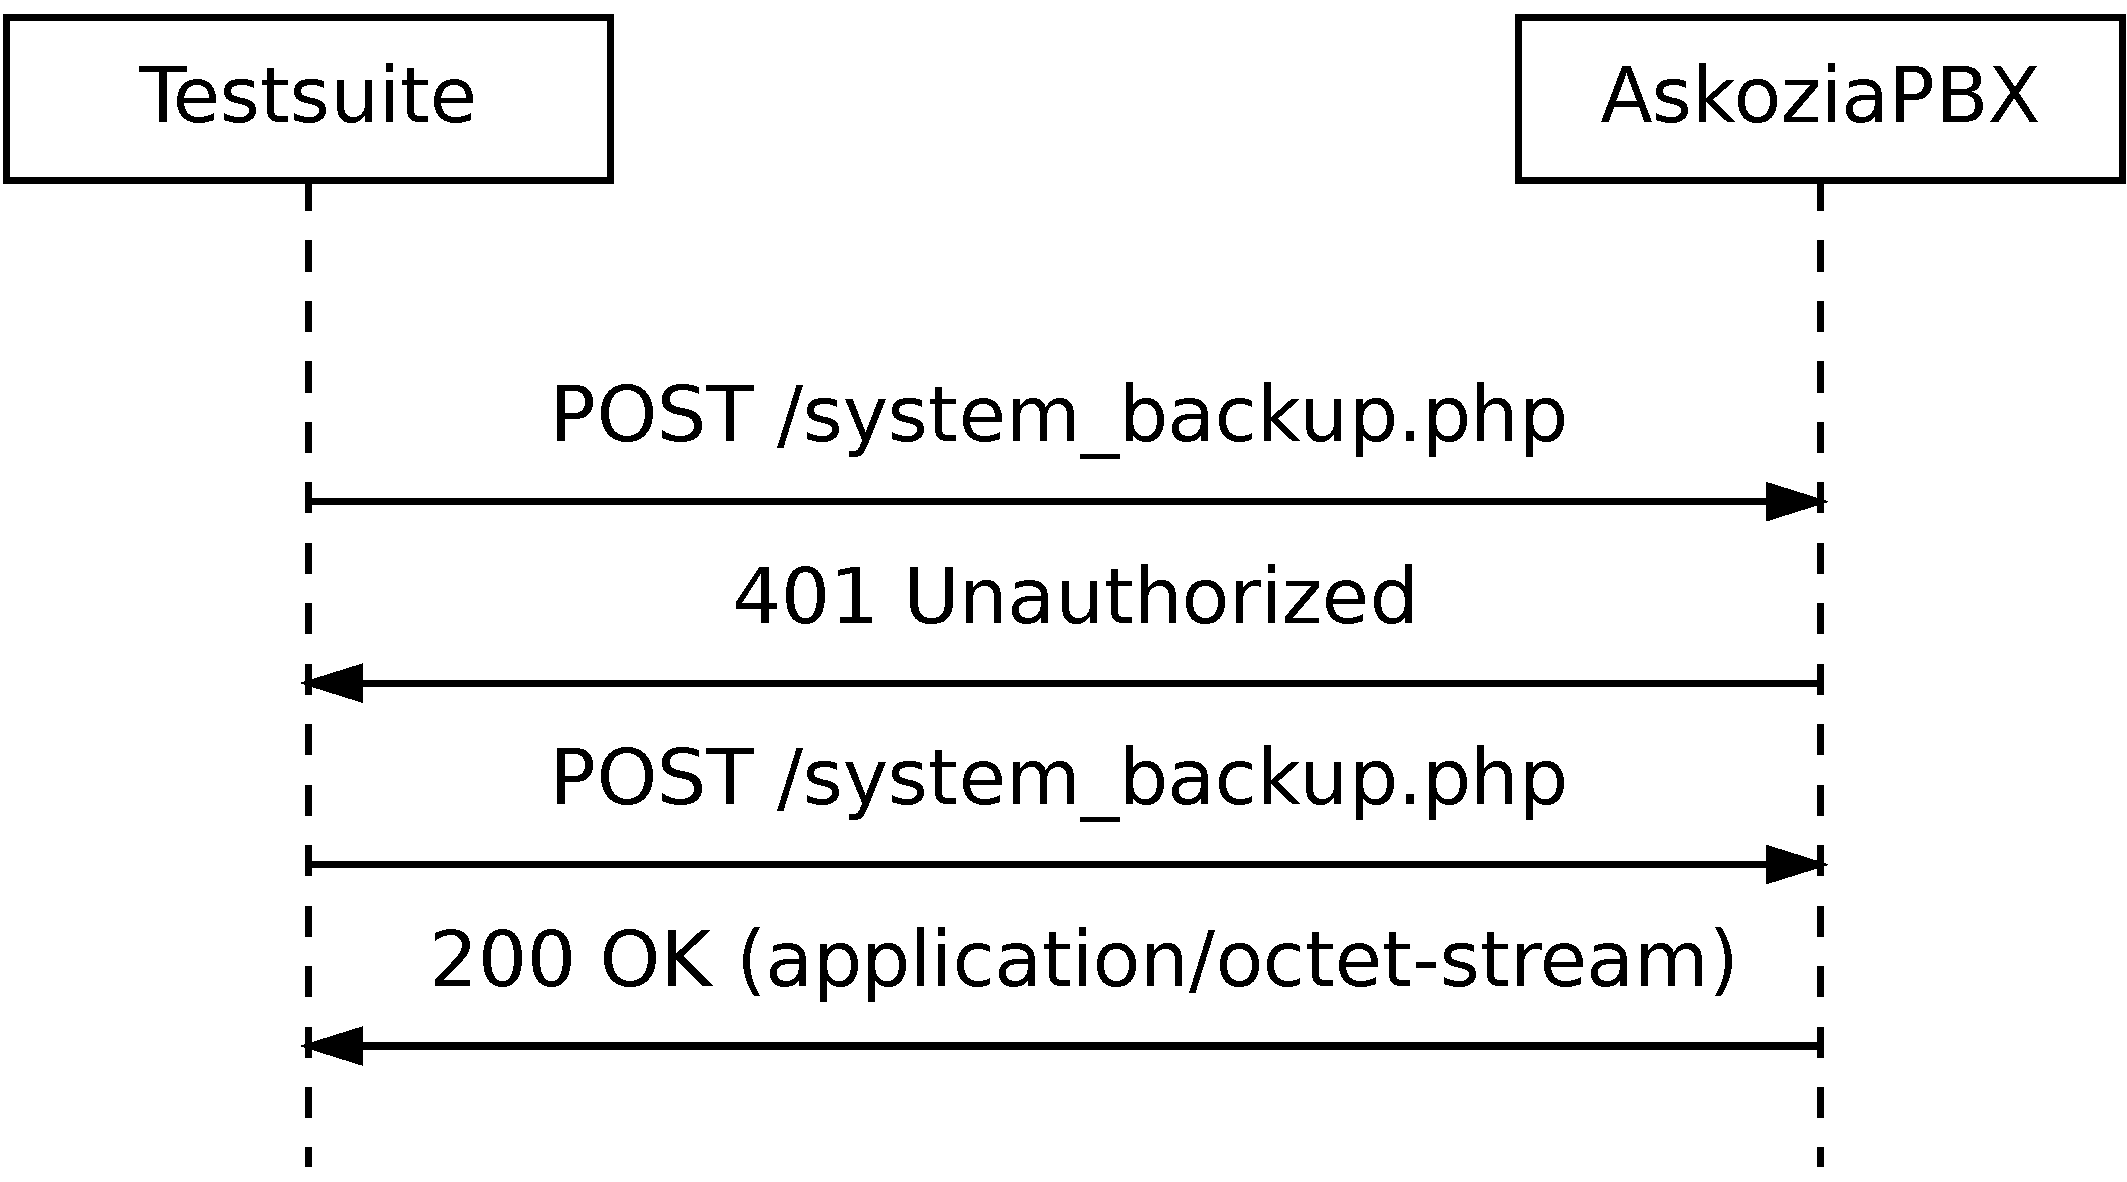
\includegraphics [width=11cm] {config-2}
\caption {Dataflow of configfile download}
\end{figure}

The ``200 OK'' message sent by Askozia includes the configfile in xml format.

\subsection{Users}

\subsection{Conference-Rooms}

